\documentclass[a4paper]{article}
\usepackage{student}
\usepackage{graphicx}
\usepackage{mathrsfs}
\usepackage{cancel}

% Metadata
\date{\today}

%-------------------------------%
% Other details
% TODO: Fill these
%-------------------------------%
\title{Taller 2}
\setmembername{Cristian Camilo Pérez Puentes} 

%-------------------------------%
% Add / Delete commands and packages
% TODO: Add / Delete here as you need
%-------------------------------%
\usepackage{amsmath,amssymb,bm}
\usepackage[spanish]{babel}

% Custom your usual commands here. Renew these.
\newcommand{\KL}{\mathrm{KL}}
\newcommand{\R}{\mathbb{R}}
\newcommand{\E}{\mathbb{E}}
\newcommand{\T}{\top}
\newcommand{\expdist}[2]{%
        \normalfont{\textsc{Exp}}(#1, #2)%
    }
\newcommand{\expparam}{\bm \lambda}
\newcommand{\Expparam}{\bm \Lambda}
\newcommand{\natparam}{\bm \eta}
\newcommand{\Natparam}{\bm H}
\newcommand{\sufstat}{\bm u}

% Main document
\begin{document}
    % Add header
    \header{}

    % Use `answer` environment to add solutions
    % \begin{answer}[Question 1.1] for example starts an environment formatted
    % for Question 1.1
    \begin{align*}
C_V=\left(\frac{\partial U}{\partial T}\right)_V ,\quad C_V=&\left(\frac{\mathrm{d} Q}{d T}\right)_V, \quad B=-V\left(\frac{\partial P}{\partial V}\right)_T \\
C_P=\left(\frac{\mathrm{d} Q}{d T}\right)_P&,\quad C_P=\left(\frac{\mathrm{d} Q}{d T}\right)_P \\
\beta=\frac{1}{V}\left(\frac{\partial V}{\partial T}\right)_P&,\quad \kappa=-\frac{1}{V}\left(\frac{\partial V}{\partial P}\right)_T \\
\left(\frac{\partial x}{\partial y}\right)_z=\frac{1}{(\partial y / \partial x)_z},\quad &\left(\frac{\partial x}{\partial y}\right)_z\left(\frac{\partial y}{\partial z}\right)_x\left(\frac{\partial z}{\partial x}\right)_y=-1 .
\end{align*}
    1.Consideremos que la energía interna de un sistema termodinámico sea una función de T y P,
    obtenga las siguientes ecuaciones:
    \begin{itemize}
        \item  $\quad\left(\frac{\partial U}{\partial T}\right)_P=C_P-P V \beta$.
        \item $\left(\frac{\partial U}{\partial P}\right)_T=P V \kappa-\left(C_P-C_V\right) \frac{\kappa}{\beta}$.
    \end{itemize}
    \begin{answer}[Problema 1]
        \begin{itemize}
            \item[a.]Dado que la energia interna es funcion de T y P, entonces:
            \begin{equation}
                U=U(T,P)
            \end{equation}
            Por lo tanto, la diferencial total de U es:
            \begin{equation}
                dU=\left(\frac{\partial U}{\partial T}\right)_P dT+\left(\frac{\partial U}{\partial P}\right)_T dP
            \end{equation}
            Por otro lado de la primera ley de la termodinamica tenemos que:
            \begin{align*}
                d Q = dU + PdV &=\left( \frac{\partial U}{\partial T} \right)_P dT + \left( \frac{\partial U}{\partial P} \right)_T dP + PdV \quad \Rightarrow\\
                & \Rightarrow \left(
                    \frac{dQ}{dT}
                \right)_P = \left( \frac{\partial U}{\partial T} \right)_P + P \left( \frac{\partial V}{\partial T} \right)_P\\
                & \Rightarrow \left(
                    \frac{dQ}{dT}
                    \right)_P = \left( \frac{\partial U}{\partial T} \right)_P + PV \frac{1}{V} \left( \frac{\partial V}{\partial T} \right)_P\\
                & \Rightarrow 
                        C_P = \left( \frac{\partial U}{\partial T} \right)_P + PV \beta\\
                & \Rightarrow \left(
                    \frac{\partial U}{\partial T}
                    \right)_P = C_P - PV \beta
            \end{align*}   
    
            Donde como se realiza $\frac{dQ}{dT}$ a volumen constante entonces 
    
            $$\left(\frac{dV}{dT}\right)_P = \left(\frac{\partial V}{\partial T}\right)_P$$  
            \item [b.] De forma analoga paratiendo de la expresion 
            \begin{align*}
                d Q = dU + PdV &=\left( \frac{\partial U}{\partial T} \right)_P dT + \left( \frac{\partial U}{\partial P} \right)_T dP + PdV \quad \Rightarrow\\
                & \Rightarrow \left(
                    \frac{dQ}{dT}
                \right)_V = \left( \frac{\partial U}{\partial T} \right)_P +  \left( \frac{\partial U}{\partial P} \right)_T \left( \frac{\partial P}{\partial T} \right)_V\\
                & \Rightarrow 
                C_V = C_P - PV \beta - \left( \frac{\partial U}{\partial P} \right)_T \left( \frac{\partial P}{\partial V} \right)_T \left( \frac{\partial V}{\partial T} \right)_P\\
                & \Rightarrow
                    \left( \frac{\partial U}{\partial P} \right)_T = \frac{C_P - PV - C_V}{\left( \frac{\partial P}{\partial V} \right)_T \left( \frac{\partial V}{\partial T} \right)_P}\\
                & \Rightarrow
                    \left( \frac{\partial U}{\partial P} \right)_T = (C_P - PV\beta - C_V)\left( \frac{\partial V}{\partial P} \right)_T \left( \frac{\partial T}{\partial V} \right)_P\\
                & \Rightarrow
                    \left( \frac{\partial U}{\partial P} \right)_T = -(C_P - PV\beta - C_V)\kappa \frac{1}{\beta}\\            \end{align*}\\
        \end{itemize}
        
    \end{answer}
    2. Tomando $\mathrm{U}$ como una función de P y V, obtenga las siguientes ecuaciones:

\begin{align*}
(a)&\quad \mathrm{d} Q=\left(\frac{\partial V}{\partial P}\right)_V d P+\left[\left(\frac{\partial U}{\partial V}\right)_P+P\right] d V.\\
(b)&\quad \left(\frac{\partial U}{\partial P}\right)_V=\frac{C_V \kappa}{\beta}.\\
(c)&\quad \left(\frac{\partial U}{\partial V}\right)_P=\frac{C_P}{V \beta}-P.\\    
\end{align*}
    \begin{answer}
        Si consideramos la energia interna como funcion de $P, V$ es decir $U = U(P,V)$ entonces de la primera ley de la termodinamica para sistema hidrostatico:
    \begin{align*}
        dQ = dU + PdV  \quad (2.1)
    \end{align*}
    \begin{itemize}
        \item [a.]  Como $U = U(P,V)$ entonces:
        \begin{align*}
            dU = \left( \frac{\partial U}{\partial P} \right)_V dP + \left( \frac{\partial U}{\partial V} \right)_P dV \quad (2.2)       
       \end{align*}
       Reemplazando (2.2) en (2.1) tenemos que:
       \begin{align*}
           dQ &= \left( \frac{\partial U}{\partial P} \right)_V dP + \left( \frac{\partial U}{\partial V} \right)_P dV + PdV \\
            &= \left( \frac{\partial U}{\partial P} \right)_V dP + \left[ \left( \frac{\partial U}{\partial V} \right)_P + P \right] dV \quad (2.3)
        \end{align*}     
    \end{itemize} 
    \begin{itemize}
        \item [b.] De (2.3)
        \begin{align*}
            \left(
                \frac{dQ}{dT} 
                \right)_V = \left( \frac{\partial U}{\partial P} \right)_V \left( \frac{dP}{dT}\right)_V \quad  (2.4)
        \end{align*}
        Y como la ecuacion de estado esta en terminos de $P$ y $V$ entonces:
        \begin{align*}
            dT = \left( \frac{\partial T}{\partial P} \right)_V dP + \left( \frac{\partial T}{\partial V} \right)_P dV \quad \Rightarrow \quad \left( \frac{dT}{dP} \right)_V = \left( \frac{\partial T}{\partial P} \right)_V
        \end{align*}
        Luego (2.4) queda:
        \begin{align*}
            \left(
                \frac{dQ}{dT} 
                \right)_V &= \left( \frac{\partial U}{\partial P} \right)_V \left( \frac{\partial T}{\partial P}\right)_V \\
                &= -\left( \frac{\partial U}{\partial P} \right)_V \left( \frac{\partial T}{\partial V}\right)_P \left( \frac{\partial V}{\partial P}\right)_V \\
                &= \left( \frac{\partial U}{\partial P} \right)_V \frac{\beta}{\kappa} = C_V \quad  \Rightarrow
        \end{align*}
        \begin{align*}
            \left( \frac{\partial U}{\partial P} \right)_V = \frac{C_V \kappa}{\beta}
        \end{align*}

        Haciendo uso de  
        \begin{align*}
            C_V = \left( \frac{\partial U}{\partial T} \right)_V  = \left(\frac{dQ}{dT}\right)_V 
        \end{align*}
        \item [c.] De (2.3)

        \begin{align*}
            \left(
                \frac {dQ}{dT}
        \right)_P &= \left( \frac{\partial U}{\partial V} \right)_P \left( \frac{\partial V}{\partial T} \right)_P + P \left( \frac{\partial V}{\partial T} \right)_P\\
        &= \left( \frac{\partial U}{\partial V} \right)_P V \beta + P V \beta = C_P \quad \Rightarrow
        \end{align*}
        \begin{align*}
            \left( \frac{\partial U}{\partial V} \right)_P V\beta = C_P - PV\beta \quad \Rightarrow \quad \left( \frac{\partial U}{\partial V} \right)_P = \frac{C_P}{V\beta} - P
        \end{align*}
        Donde se ha hecho uso de la ecuacion de estado es funcion de $P$ y $V$.
        $$ \left(
            \frac {dT}{dV}
        \right)_P = \left( \frac{\partial T}{\partial V} \right)_P$$
        \end{itemize}
    \end{answer}
    3. Un mol de un gas obedece a la ecuación de estado de van der Waals:
\begin{align*}
\left(P+\frac{a}{v^2}\right)(v-b)=R T    
\end{align*}
Donde a, b y R son constantes, demuestre que
\begin{align*}
    c_p-c_v=\frac{R}{1-2 a(1-b / V)^2 / V R T}
\end{align*}
    \begin{answer}[Punto 3]
    Si consideramos la enegia interna como funcion de $T$ y $V$ es decir $U = U(T,V)$ entonces:
    \begin{align*}
        dU = \left( \frac{\partial U}{\partial T} \right)_V dT + \left( \frac{\partial U}{\partial V} \right)_T dV \quad (3.1)
    \end{align*}
    entonces Reemplazando (3.1) en (2.1) tenemos que:
    \begin{align*}
        &dQ = \left( \frac{\partial U}{\partial T} \right)_V dT + \left( \frac{\partial U}{\partial V} \right)_T dV + PdV \quad (3.2)\quad\\ 
        &\Rightarrow \quad  C_P = \left( \frac{dQ}{dT} \right)_P = \left( \frac{\partial U}{\partial T} \right)_V + \left( \frac{\partial U}{\partial V} \right)_T \left( \frac{\partial V}{\partial T} \right)_P + P \left( \frac{\partial V}{\partial T} \right)_P\\
        &\Rightarrow \quad C_V = \left( \frac {dQ}{dT} \right)_V = \left( \frac{\partial U}{\partial T} \right)_V \quad \Rightarrow
    \end{align*}
    \begin{align*}
        C_P - C_V = \left[ \left( \frac{\partial U}{\partial V} \right)_T + P \right] \left( \frac{\partial V}{\partial T} \right)_P \quad (3.3)
    \end{align*}
    Tambien de (3.2)
    \begin{align*}
        \left(\frac{dQ}{dV}\right)_T = \left( \frac{\partial U}{\partial V} \right)_T + P \quad &\Rightarrow \quad \left( \frac{\partial U}{\partial V} \right)_T = \left(\frac{dQ}{dV}\right)_T - P\\
        &\Rightarrow \quad \left( \frac{\partial U}{\partial V} \right)_T = T \left( \frac{\partial S}{\partial V} \right)_T - P \quad dQ = TdS \quad \text{$T$ constante}\\
        &\Rightarrow \quad \left( \frac{\partial U}{\partial V} \right)_T = T\left( \frac{\partial P}{\partial T} \right)_V - P \quad (3.4) \quad \text{$\left( \frac{\partial S}{\partial V} \right)_T = \left( \frac{\partial P}{\partial T} \right)_V$}
    \end{align*}
    De (3.3) y (3.4)
    \begin{align*}
        C_P - C_V &= \left[ T\left( \frac{\partial P}{\partial T} \right)_V - P + P \right] \left( \frac{\partial V}{\partial T} \right)_P \quad &\Rightarrow \quad C_P - C_V = T\left( \frac{\partial P}{\partial T} \right)_V \left( \frac{\partial V}{\partial T} \right)_P\\
        &=T \left( \frac{\partial P}{\partial T} \right)_V \left( \frac{\partial V}{\partial T} \right)_P \\
     \end{align*}
    
    Del taller anterior sabemos que:
    \begin{align*}
        \left( \frac{\partial P}{\partial T} \right)_V = \frac{R}{V-b} \quad \text{y} \quad \left( \frac{\partial V} {\partial T}\right)_P  = \frac{RV^3}{2ab - aV + PV^3}
    \end{align*}
    Por lo tanto 

    \begin{align*}
        C_P - C_V &= T \frac{R}{V-b} \frac{RV^3}{2ab - aV + PV^3} \\
        &= \frac{R^2TV^3}{2(ab - aV)(V-b) +(V-b)\left(\frac a{V^2} + P\right)V^3}\\
        &= \frac{R^2TV^3}{-2a(V - b)(V-b) +RT V^3}\\
        &= \frac{R}{1 -\frac{2a(V- b)^2}{RTV^3}}\\
    \end{align*}
    \end{answer}
    4. La ecuación de estado de un sólido monoatómico es
$$
P v+f(v)=\Gamma u \quad (4.1)
$$
donde $v$ es el volumen molar, $\Gamma$ es la constante de Grüneisen y u es la energía interna molar debida a las vibraciones de la red. Demostrar que
$$
\Gamma=\frac{\beta v}{c_V \kappa}
$$
donde $\kappa$, es la compresibilidad isotérmica. Esta ecuación, conocida como relación de Grüneisen, juega un papel importante en la teoría del estado sólido.
    \begin{answer}
        Dado que la ecuacion de estado representa un sistema hidrostatico con $u = u(P,v)$ entonces:

        \begin{align*}
            du = \left( \frac{\partial u}{\partial P} \right)_v dP + \left( \frac{\partial u}{\partial v} \right)_P dv \quad (4.2)
        \end{align*}
        Donde de (4.1):
        \begin{align*}
            \left(\frac {\partial u}{\partial P}\right)_v &= \left(
                \frac{\partial}{\partial P} \left(  P\frac v\Gamma + \frac{f(v)}\Gamma \right)
            \right)_v \\ 
            &= \frac{v}{\Gamma} 
        \end{align*}
        \begin{align*}
            \left(\frac {\partial u}{\partial v}\right)_P &= \left(
                \frac{\partial}{\partial v} \left(  P\frac v\Gamma + \frac{f(v)}\Gamma \right)
            \right)_P\\
            &= \left( \frac{\partial}{\partial v} \left( \frac{f(v)}\Gamma \right) \right)_P + \frac P \Gamma\left( \frac{\partial}{\partial v} \left(  v \right) \right)_P\\
            &= \frac 1\Gamma \left( \frac{\partial f(v)}{\partial v} \right)_P + \frac P \Gamma\\
        \end{align*}
        Reemplazando en (4.2) tenemos que:
        \begin{align*}
            \Gamma dU = v dP + \left( \frac{\partial f(v)}{\partial v} \right)_P dv + P dv \quad  &\Rightarrow \quad \left(\frac {\partial u}{\partial T}\right)_v = \frac v\Gamma \left( \frac{\partial P}{\partial T} \right)_v = c_V\\
            &\Rightarrow \quad c_V =- \frac v\Gamma \left( \frac{\partial P}{\partial v } \right)_T \left( \frac{\partial v}{\partial T} \right)_v\\
            &\Rightarrow \quad c_V = \frac v\Gamma \frac \beta \kappa \\
            &\Rightarrow \quad \Gamma = \frac{\beta v}{c_V \kappa}
        \end{align*}
       
    \end{answer}
    5. En el caso de un gas paramagnético, derive la ecuación
$$
dQ=\left(\frac{\partial U}{\partial T}\right)_{V, \mathscr{M}} d T+\left[\left(\frac{\partial U}{\partial V}\right)_{\mathscr{M}, T}+P\right] d V+\left[\left(\frac{\partial U}{\partial \mathscr{M}}\right)_{T, V}-\mu_0 \mathscr{H}\right] d \mathscr{M}
$$
    \begin{answer}[Punto 5]
        Dado que este es este es un sistema hidrostatico y paramagnetico la primera ley de la termodinamica toma la forma:
        \begin{align*}
            dQ = dU - PdV + \mu_0 \mathscr Hd\mathscr{M} \quad (5.1)
        \end{align*}
        Donde las variables termodinamicas asociadas a un sistema hidrostatico son $T,~P,~V$ y las variable termodinamicas asociadas a un sistema paramagnetico son $T, \mathscr{H}, \mathscr{M}$.
        Coordenadas de las cuales solo tres son independientes, siendo las mas convinientes $T,V,\mathscr M$, por lo tanto 
        $$dU = dU(T,V, \mathscr{M}) =  \left(\frac{\partial U}{\partial T}\right)_{V, \mathscr{M}} dT +\left(\frac{\partial U}{\partial V}\right)_{T, \mathscr{M}} dV + \left(\frac{\partial U}{\partial \mathscr{M}}\right)_{T,V} d\mathscr{M}$$ 

        Reemplazando el diferencial de energia interna en (5.1) entonces:

        \begin{align*}
            dQ &=  \left(\frac{\partial U}{\partial T}\right)_{V, \mathscr{M}} dT +\left(\frac{\partial U}{\partial V}\right)_{T, \mathscr{M}} dV + \left(\frac{\partial U}{\partial \mathscr{M}}\right)_{T,V} d\mathscr{M} - PdV + \mu_0 \mathscr H d\mathscr M\\
             &= \left(\frac{\partial U}{\partial T}\right)_{V, \mathscr{M}} dT + \left[\left(\frac{\partial U}{\partial V}\right)_{T, \mathscr{M}} - P \right]dV + \left[\left(\frac{\partial U}{\partial \mathscr{M} } \right)_{T,V} + \mu_0\mathscr H\right] d\mathscr M
        \end{align*}
    \end{answer}
    6. Demuestre que el calor transferido durante un proceso cuasiestático infinitesimal de un gas ideal se puede escribir
$$
\mathrm{d} Q=\frac{C_V}{n R} V d P+\frac{C_P}{n R} P d V
$$
Aplicando esta ecuación a un proceso adiabático, demuestre que $P V^{\gamma}=$ const.
    \begin{answer}[Punto 6]
        Dado que la ecuacion de estado para un gas ideal es:
        \begin{align*}
            PV = nRT \quad (6.1) \quad \text{con}  \quad \left(\frac{\partial U}{\partial V}\right)_T = 0 \quad \text{y} \quad \left(\frac{\partial U}{\partial P}\right)_V = 0
        \end{align*}
        Por lo que la energia interna cumple que $U = U(T)$
        \begin{align*}
            dU = \left(\frac{\partial U}{\partial T}\right)_V dT   \quad \Rightarrow \quad C_V =  \frac{dU}{dT}= \left(\frac{\partial U}{\partial T}\right)_V \quad (6.2)
        \end{align*}\
        Por otro lado de la primera ley de la termodinamica para el gas ideal, desde las ecuacion (2.1) y (6.2), toma la forma:
        \begin{align*}
            dQ = \left(\frac{\partial U}{\partial T}\right)_V dT + PdV  = C_VdT + PdV \quad (6.3)
        \end{align*}
        Donde 
        \begin{align*}
            dT &= \left(\frac{\partial T}{\partial V}\right)_P dV + \left(\frac{\partial T}{\partial P}\right)_V dP\\
            &= \frac{P}{nR}dV + \frac{V}{nR}dP \quad 
        \end{align*}
        Reemplazando en (6.3) tenemos que:
        \begin{align*}
            dQ = C_V \left( \frac{P}{nR}dV + \frac{V}{nR}dP \right) + PdV \quad &\Rightarrow \quad dQ = \frac{C_V}{nR}PdV + \frac{C_V}{nR}VdP + PdV\\
            &\Rightarrow \quad dQ = \frac{C_V}{nR}VdP + \left( \frac{C_V}{nR} + 1 \right)PdV\\
            &\Rightarrow \quad dQ =  \frac{C_V}{nR}VdP + \left( \frac{C_V + nR}{nR}\right)PdV\\
            &\Rightarrow \quad dQ =  \frac{C_V}{nR}VdP +  \frac{C_P}{nR} PdV \quad (6.4)\\
        \end{align*}
        Donde se uso que $C_P - C_V = nR$ para un gas ideal.
        Ahora si consideramos tambien que es gas esta sometido a un proceso adiabatico entonces de (6.4)
        \begin{align*}
            dQ = 0 \quad &\Rightarrow \quad \frac{C_V}{nR}VdP +  \frac{C_P}{nR} PdV = 0\\
            &\Rightarrow \quad \frac{C_V}{nR}VdP = - \frac{C_P}{nR} PdV\\
            &\Rightarrow \quad \frac{C_P}{C_V}\frac{dV}{V} = -\frac{dP}{P}\\
            &\Rightarrow \quad \gamma \ln(V) = -\ln(P) + C\\
            &\Rightarrow \quad \ln(V^\gamma) = \ln(P^{-1}) + C\\
            &\Rightarrow \quad V^\gamma = P^{-1}e^C\\
            &\Rightarrow \quad PV^\gamma = e^C = \text{constante}\\
        \end{align*}

    \end{answer}
    7. Un mol de un sistema paramagnético ideal obedece la ley de Curie.
$$
\mathscr{M} =\frac{C_{C} \mathscr H}{T}
$$
Donde $\mathscr M$ es la magnetización y $\mathscr H$ es un campo magnético externo, con constante de Curie $C_C$. Suponga que la energía interna $U$ es función de $T$ únicamente, de modo que $\mathrm{dU}=\mathrm{C}_{\mathrm{V},\mathscr M}  \mathrm{dT}$, donde $\mathrm{C}_{\mathrm{v}, \mathscr{M}}$ es una capacidad calorífica a volumen y magnetización constantes. Demostrar que la ecuación de la familia de superficies adiabáticas es
$$
\frac{C_{V, \mathscr M}}{n R} \ln T+\ln V=\frac{\mu_0 \mathscr M^2}{2 n R C_C}+\ln A,
$$
Donde A es una constante.
    \begin{answer}[Punto 7]
        Dado que este es un sistema paramagnetico e hidrostatico  con funcion de energia interna $U = U(T)$ tal que $dU = C_{V, \mathscr{M}} dT$, entonces de el ejercicio 5 tenemos que la primera ley de la termodinamica queda:
        \begin{align*}
            dQ = C_{V, \mathscr{M}} dT + PdV - \mu_0 \mathscr{H} d\mathscr{M} \quad (7.1) \quad \text{donde } \quad \left(\frac{\partial U}{\partial V}\right)_{\mathscr{M},T} = 0 \quad \text{y} \quad \left(\frac{\partial U}{\partial \mathscr{M}}\right)_{T,V} = 0 
        \end{align*}
        Y para un proceso adiabatico $dQ = 0$ entonces de (7.1) tenemos que:
        \begin{align*}
            0 = C_{V, \mathscr{M}} dT + PdV - \mu_0 \mathscr{H} d\mathscr{M} \quad &\Rightarrow \quad C_{V, \mathscr{M}} + P\frac{dV}{dT}= \mu_0 \mathscr{H}\frac{d\mathscr{M}}{dT} \quad (7.2)\\
        \end{align*}
        Donde para un gas ideal y para un sistema paramagnetico se cumplem respectivamente que:
        \begin{align*}
            PV = nRT \quad \text{y} \quad \mathscr{M} = \frac{C_C \mathscr{H}}{T} \quad &\Rightarrow \quad V = \frac{nRT}{P} \quad \text{y} \quad \frac{d\mathscr{M}}{dT} = -\frac{C_C\mathscr H}{T^2}\\
        \end{align*}
        Reemplazando en (7.2)
        \begin{align*}
            C_{V, \mathscr{M}} + P\frac{dV}{dT}= \mu_0 \mathscr{H}\frac{d\mathscr{M}}{dT} \quad &\Rightarrow \quad \frac{nRT}{V} dV =  -\left( C_{V,\mathscr M} +  \mu_0 \mathscr H\frac{C_C\mathscr H}{T^2} \right)dT\\
            & \Rightarrow \quad \frac{nR}{V} dV + C_{V,\mathscr M}\frac{dT}{T}  +  \mu_0C_C\mathscr H^2 \frac{dT}{T^3} = 0\\ 
            & \Rightarrow \quad nR \ln(V) + C_{V,\mathscr M} \ln(T) -  \frac{\mu_0 C_C\mathscr H^2 }{2T^2}  = C\\ 
            & \Rightarrow \quad nR \ln(V) + C_{V,\mathscr M} \ln(T) -  \frac{\mathscr{M}^2 }{2 C_C}  = C \quad  \frac{\mathscr{H}^2}{T^2} = \frac{ \mathscr{M}^2}{C_C^2}\\
            & \Rightarrow \quad \frac{C_{V,\mathscr M}}{nR} + \ln(V)  = \frac{\mathscr{M}^2}{2 C_C nR} + \ln(A) \quad \text{donde } A = e^C = \text{constante}\\
        \end{align*}

    \end{answer}
    8. La figura 1 , se representa un diagrama $PV$ simplificado del ciclo de gas ideal de Joule. Todos los procesos son cuasi-estáticos y $\mathrm{C_P}$ es constante. Demuestre que la eficiencia térmica de un motor que realiza este ciclo es
$$
\eta=1-\left(\frac{P_{\mathbf{1}}}{P_2}\right)^{(\gamma-1) / \gamma}
$$
figura 1. Ciclo de gas ideal Joule

\begin{figure}[h]
    \centering
    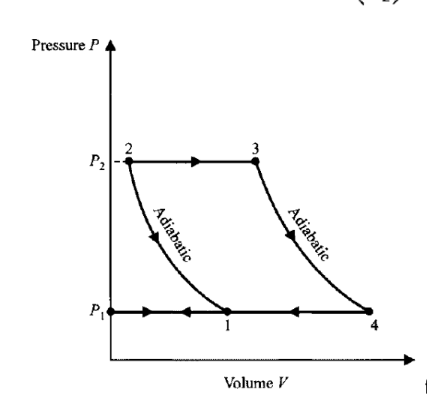
\includegraphics[width=0.5\textwidth]{diagrama.png}
    \label{fig:figura1}    
\end{figure}
    \begin{answer}[Punto 8]
        Dado que durante todo el ciclo se tiene que durante proceso isobarico se cumple
        \begin{align*}
            C_P = \left( \frac{dQ}{dT} \right)_P  \quad &\Rightarrow \quad Q_{12} = C_P \int _{T_1}^{T_2} dT = C_P (T_2 - T_1) \quad (8.1.1) \quad \text{si el calor es absorbido}\\
            &\Rightarrow \quad Q_{12} = -C_P \int _{T_1}^{T_2} dT = -C_P (T_2 - T_1) \quad (8.1.2) \quad \text{si el calor es cedido}\\
        \end{align*}
        Como de $1 \rightarrow 2$ es un proceso adiabatico entonces $dQ = 0$ y por lo tanto
        \begin{align*}
            P_1V_1^\gamma = P_2V_2^\gamma \quad (8.2)
        \end{align*}
        De $2 \rightarrow 3$ es un proceso isobarico el calor absorbido por el sistema es:
        \begin{align*}
            Q_{2\rightarrow 3} = C_P \Delta T = C_P (T_3 - T_2) \quad \text{Aplicando (8.1.1)}
        \end{align*}
        De $3 \rightarrow 4$ es un proceso adiabatico:
        \begin{align*}
            P_1V_4^\gamma = P_2V_3^\gamma \quad (8.3)
        \end{align*}
        Por ultimo de $4 \rightarrow 1$ es un proceso isocorico por lo que el calor absorbido es
        \begin{align*}
            Q_{4\rightarrow 1} = C_V \Delta T = C_P (T_4 - T_1) \quad \text{Aplicando (8.1.2)}
        \end{align*}
        Dividiendo ahora las expresiones (8.2) y (8.3) tenemos que:
        \begin{align*}
            \frac{V_1^\gamma}{V_4^\gamma} = \frac{V_2^\gamma}{V_3^\gamma} \quad &\Rightarrow \quad \frac{V_1}{V_4} = \frac{V_2}{V_3}\\
            & \Rightarrow \quad V_1 V_3 = V_2 V_4 \quad (8.4)
        \end{align*}

        Por la definicion de eficiencia:
        \begin{align*}
            \eta &= 1 - \frac{Q_{4\rightarrow 1}}{Q_{2\rightarrow 3}} = 1 - \frac{C_P (T_4 - T_1)}{C_P (T_3 - T_2)}\\
            &= 1 - \frac{T_3 - T_2}{T_4 - T_1} = 1 - \frac{\frac{P_1 V_4}{nR} - \frac{P_1 V_1}{nR}}{\frac{P_2 V_3}{nR}  -\frac{P_2 V_2}{nR}} \quad \text{Aplicando (6.1)}\\
            &= 1 - \frac{P_1V_4 -P_1 V_1 }{P_2 V_3 - P_2 V_2} = 1 - \frac{P_1}{P_2} \frac{V_3 - V_2}{V_1 - V_4}\\
            &= 1 - \left( \frac{V_2}{V_1} \right)^{\gamma} \frac{V_4 - V_1}{V_3 - V_2} = \left( \frac{V_2}{V_1} \right)^{\gamma-1} \frac{V_4V_2 - V_1V_2}{V_3V_1 - V_2V_1}  \quad \text{Aplicando (8.2)}\\
            &= 1 - \left( \frac{V_2}{V_1} \right)^{\gamma-1} \frac{ V_3 V_1 - V_2 V_1}{V_3 V_1 - V_2 V_1} = 1 - \left( \frac{V_2}{V_1} \right)^{\gamma-1} \quad \text{Aplicando (8.4)}\\
            &= 1 - \left( \frac{V_2^\gamma}{V_1^\gamma} \right)^{\frac{\gamma-1}{\gamma}} = 1 - \left( \frac{P_1}{P_2} \right)^{\frac{\gamma-1}{\gamma}} \quad \text{Aplicando (8.2)}\\
        \end{align*}
    \end{answer}
    9. (a) Deduzca la expresión para la eficiencia de un motor de Carnot directamente de un diagrama TS (Temperatura vs Entropía). (b) Compare las eficiencias de los ciclos A y B de la Figura 2.
figura 2.

\begin{figure}[h]
    \centering
    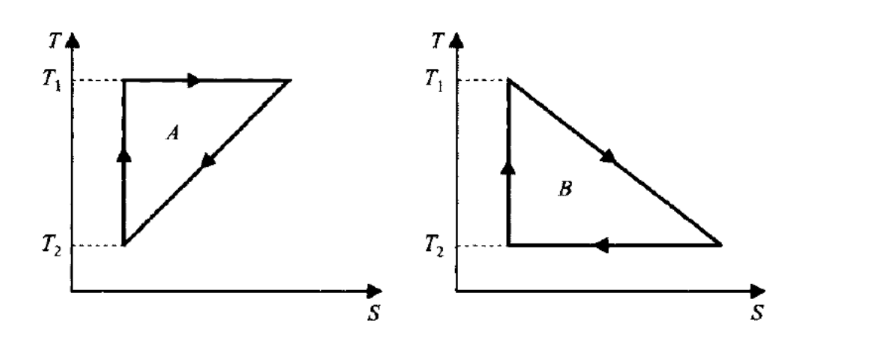
\includegraphics[width=0.5\textwidth]{diagram2.png}
    
    \label{fig:figura2}
\end{figure}
    \begin{answer}
        Dado que el calor y la entropia estan relacionada por la ecuacion:
        \begin{align*}
            dQ = TdS \quad (9.1)
        \end{align*}
        \begin{itemize}
            \item [a.] En un diagrama $PV$ del un ciclo de Carnot consiste de dos curvas adiabaticas, la cuales en un digrama $TS$ consisten de dos lineas rectas que representa la entropia constante para distintos valores de la temperatura, pero a difrencia del diagrama anterior, este diagrama tambien consistira de dos curvas isotermicas representadas por dos lineas horizontales conectando las dos lineas adiabaticas, como se ve en la figura 1
            De esta manera la eficiencia va estar dada por 
    
            \begin{align*}
                \eta &= 1 - \frac{Q_{4\rightarrow 1}}{Q_{2\rightarrow 3}} = 1 - \frac{|Q_L|}{|Q_H|}\\
                &= 1 - \frac{T_L \Delta S_L}{T_H \Delta S_H} \quad \text{Aplicando (9.1)}\\
                &= 1 - \frac{T_L}{T_H} \quad 
            \end{align*}
            Esto ultimo debido a que  $2\rightarrow 3 \quad \text{y} \quad 4\rightarrow 1 \quad \text{son isoentropicos es decir} \quad S_3 = S_2 \quad \text{y} \quad S_4 = S_1 \Rightarrow \Delta S_L = \Delta S_H$
            \item [b.] Del diagrama de la izquierda obtenemos que:
            \begin{align*}
                |Q_H| &= T_1 (S_ 1- S_2)= T_1 \Delta S_H \\
                |Q_L| &= -\int_{S_1}^{S_2} T(S) dS = -\int_{S_1}^{S_2} \left( \frac{T_1 - T_2 }{S_1 - S_2}S - \frac{T_1S_2 - T_2S_1}{S_1 - S_2}\right)dS \\
                &= -\left( \frac{T_1 - T_2 }{S_1 - S_2} \frac{S_2^2 - S_1^2}{2} - \frac{T_1S_2 - T_2S_1}{S_1 - S_2} (S_2 - S_1)\right)\\
                &=-\left( T_2 - T_1 \frac{S_2 + S_1}{2} + T_1S_2 - T_2S_1\right)\\
                &= - \left(\frac 12 T_2S_1 + \frac 12 T_2 S_2 - \frac 12 T_1 S_1 - \frac 12 T_1 S_2  + T_1S_2 -T_2S_1\right)\\
                &= - \left( -\frac 12 T_1 S_1 + \frac 12 T_1 S_2 - \frac 12 T_2 S_1 + \frac 12 T_2 S_2 \right)\\
                &= - \left( \frac 12 T_1 (S_2 - S_1) + \frac 12 T_2 (S_2- S_1) \right)\\
                &= \frac 12 (T_1 + T_2) (S_1 - S_2)\\
            \end{align*}
            De esta manera la eficiencia queda:
            \begin{align*}
                \eta_L = 1 - \frac{|Q_H|}{|Q_L|} = 1 - \frac{T_1 + T_2}{2T_1} = \frac{T_1 - T_2}{2T_1}
            \end{align*}
            Ahora del  diagrama de la derecha obtenemos que:
            \begin{align*}
                |Q_L| &= T_2 (S_ 2- S_1)\\
                |Q_H| &= \int_{S_1}^{S_2} T(S) dS = \int_{S_1}^{S_2} \left( \frac{T_2 - T_1 }{S_2 - S_1}S - \frac{T_2S_1 - T_1S_2}{S_2 - S_1}\right)dS \\
                &= \left( \frac{T_2 - T_1 }{S_2 - S_1} \frac{S_2^2 - S_1^2}{2} - \frac{T_2S_1 - T_1S_2}{S_2 - S_1} (S_2 - S_1)\right)\\
                &=\left( T_2 - T_1 \frac{S_2 + S_1}{2} - T_2S_1 + T_1S_2\right)\\
                &= \left(-\frac 12 T_1S_1 - \frac 12 T_1 S_2 + \frac 12 T_2 S_1 + \frac 12 T_2 S_2  - T_2S_1 +T_1S_2\right)\\
                &= \left( -\frac 12 T_1 S_1 + \frac 12 T_1 S_2 - \frac 12 T_2 S_1 + \frac 12 T_2 S_2 \right)\\
                &= \left( \frac 12 T_1 (S_2 - S_1) + \frac 12 T_2 (S_2- S_1) \right)\\
                &= \frac 12 (T_1 + T_2) (S_2 - S_1)\\
            \end{align*}
            Por lo que ahora la eficiencia queda:
            \begin{align*}
                \eta_R = 1 - \frac{|Q_H|}{|Q_L|} = 1 - \frac{2T_2}{T_1 + T_2} = \frac{T_1 - T_2}{T_1+T_2}
            \end{align*}
            Si realizamos la difrencia de estas dos eficiencias tenemos que:
            \begin{align*}
                \eta_L - \eta_R &= \frac{T_1 - T_2}{2T_1} - \frac{T_1 - T_2}{T_1+T_2} = \frac{(T_1 - T_2)(T_1 + T_2) - 2T_1(T_1 - T_2)}{2T_1(T_1 + T_2)}\\
                &= \frac {T_1^2 - T_2^2 - 2T_1^2 + 2T_1T_2}{2T_1(T_1 + T_2)} = \frac{-T_1^2 + 2T_1T_2 - T_2^2}{2T_1(T_1 + T_2)}\\
                &= \frac{-(T_1 - T_2)^2}{2T_1(T_1 + T_2)} < 0 
            \end{align*}
            De esta forma el ciclo de la derecha es mas eficiente que el de la izquierda.

        \end{itemize}
        
    \end{answer}

    \begin{figure}[h]
        \centering
        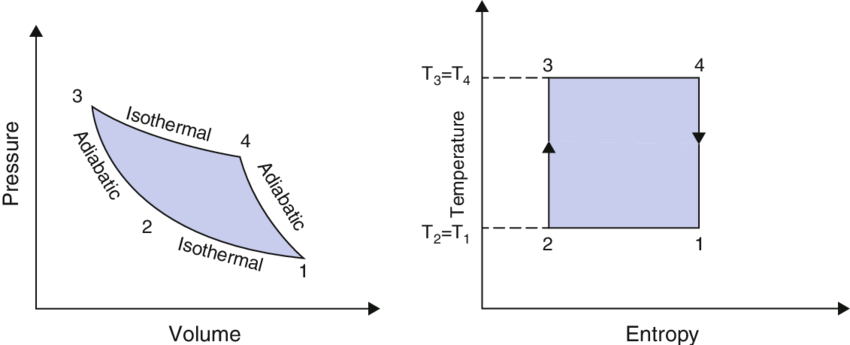
\includegraphics[width=0.5\textwidth]{Diagrama3.png}
        \caption{Diagrama $TS$ de un ciclo de Carnot}
    \end{figure}

    10. La capacidad calorífica molar a campo magnético constante de un sólido paramagnético a bajas temperaturas varía con la temperatura y el campo según la relación
$$
C_{\mathscr{H}}=\frac{B+C \mathscr{H}}{T^2}+D T^2
$$
donde B, C y D son constantes. ¿Cuál es el cambio de entropía de n moles de material cuando la temperatura cambia de $\mathrm{T_i}$ a $T_f$ mientras que $\mathscr{H}_{0}$ permanece constante en el valor $\mathscr{H_0}$ 
    \begin{answer}
        De la primera ley para un sistema paramagnetico, la cual es:
        \begin{align*}
            dQ = dU - \mu_0 \mathscr{H} d\mathscr{M} \quad (10.1)
        \end{align*}
        Donde la energia $U= U(\mathscr{M}, T)$ por lo tanto:

        \begin{align*}
            dU = \left(\frac{\partial U}{\partial \mathscr{M}}\right)_T d\mathscr{M} + \left(\frac{\partial U}{\partial T}\right)_{\mathscr{M}} dT \quad (10.2)
        \end{align*}
        entonces Reemplazando (10.2) en (10.1)
        \begin{align*}
            &dQ = \left(\frac{\partial U}{\partial \mathscr{M}}\right)_T d\mathscr{M} + \left(\frac{\partial U}{\partial T}\right)_{\mathscr{M}} dT - \mu_0 \mathscr{H} d\mathscr{M} \\
            &\Rightarrow \quad  dQ = \left(\frac{\partial U}{\partial T}\right)_{\mathscr{M}} dT + \left[\left(\frac{\partial U}{\partial \mathscr{M}}\right)_T - \mu_0 \mathscr{H} \right] d\mathscr{M}\\
            &\Rightarrow \quad  \left(\frac {dQ}{dT}\right)_{\mathscr{H}}  = \left(\frac{\partial U}{\partial T}\right)_{\mathscr{M}} + \left[\left(\frac{\partial U}{\partial \mathscr{M}}\right)_T - \mu_0 \mathscr{H} \right] \left(\frac{\partial \mathscr{M}}{\partial T}\right)_{\mathscr{H}}\\
            &\Rightarrow \quad C_{\mathscr{H}} = \left(\frac{\partial U}{\partial T}\right)_{\mathscr{M}} + \left[\left(\frac{\partial U}{\partial \mathscr{M}}\right)_T - \mu_0 \mathscr{H} \right] \left(\frac{\partial \mathscr{M}}{\partial T}\right)_{\mathscr{H}} \\ 
            &\Rightarrow \quad C_{\mathscr{H}} = \left(\frac{\partial U}{\partial T}\right)_{\mathscr{M}} + \left[\left(\frac{\partial U}{\partial \mathscr{M}}\right)_T  \left(\frac{\partial \mathscr{M}}{\partial T}\right)_{\mathscr{H}} - \mu_0 \mathscr{H}  \left(\frac{\partial \mathscr{M}}{\partial T}\right)_{\mathscr{H}} \right] \\
            &\Rightarrow \quad C_{\mathscr{H}} = \left(\frac{\partial U}{\partial T}\right)_{\mathscr{M}} + \left[-\left(\frac{\partial U}{\partial T}\right)_{\mathscr{M}}  - \mu_0 \mathscr{H}  \left(\frac{\partial \mathscr{M}}{\partial T}\right)_{\mathscr{H}} \right] \\  
            &\Rightarrow \quad C_{\mathscr{H}} = - \mu_0 \mathscr{H}  \left(\frac{\partial \mathscr{M}}{\partial T}\right)_{\mathscr{H}}\\  
        \end{align*}
        Ahora desde la ley de Curie:
        \begin{align*}
            \mathscr{M} = \frac{C_C \mathscr{H}}{T} \quad &\Rightarrow \quad \left(\frac{\partial \mathscr{M}}{\partial T}\right)_{\mathscr{H}} = -\frac{C_C \mathscr{H}}{T^2}\\
        \end{align*}
        luego:
        \begin{align*}
            C_{\mathscr{H}} = \mu_0 \mathscr{H}\frac{C_C \mathscr{H}}{T^2}
        \end{align*}
        Ahora la entropia esta definida por:
        \begin{align*}
            dQ = TdS \quad &\Rightarrow \quad \left( \frac{dQ}{dT}\right)_{\mathscr{H}} = T \left(\frac{dS}{dT}\right)_\mathscr{H}\\
            &\Rightarrow \quad C_{\mathscr{H}} = T \left(\frac{dS}{dT}\right)_{\mathscr{H}}\\
            &\Rightarrow \quad dS = \frac{C_{\mathscr{H}}}{T}dT\\
            &\Rightarrow \quad dS = \left(\frac{B+C \mathscr{H_0}}{T^2}+D T^2\right)\frac{dT}{T}\\
            &\Rightarrow \quad S = \int_{T_i}^{T_f} \left(\frac{B+C \mathscr{H_0}}{T^2}+D T^2\right)\frac{dT}{T}\\
            &\Rightarrow \quad S = \int_{T_i}^{T_f} \left(\frac{B+C \mathscr{H_0}}{T^3}+D T\right)dT\\
            &\Rightarrow \quad S = \left[-\frac{B+C \mathscr{H_0}}{2T^2}+D \frac{T^2}{2}\right]_{T_i}^{T_f}\\
            &\Rightarrow \quad S = -\frac{B+C \mathscr{H_0}}{2T_f^2}+D \frac{T_f^2}{2} + \frac{B+C \mathscr{H_0}}{2T_i^2}-D \frac{T_i^2}{2}\\
            &\Rightarrow \quad S = \frac{B+C \mathscr{H_0}}{2}\left(\frac{1}{T_i^2}-\frac{1}{T_f^2}\right)+D \left(\frac{T_f^2}{2} -\frac{T_i^2}{2}\right)\\
        \end{align*}
    \end{answer}
\end{document}